\section[More Modeling with Mechanical Energy]{More Modeling of Scenarios involving Mechanical Energy Systems}
\label{act2.2.2}

\begin{overview}
	
	\textbf{Overview:} In this activity, we will explore additional scenarios that are related to phenomena we've already discussed. Here, we add some variations to the scenarios and answer some different questions we haven't asked yet.
	
\end{overview}

\noindent\textbf{Note:} Remember Christine throwing a ball in the air in \hyperref[act2.2.1b]{Activity~\ref*{act2.2.1b}} (page\pageref*{act2.2.1b} )?

\note{Important! }{Assign one only (see activity sheet) to each \SG{}. Have each \SG{} present their response in the Whole Class Discussion. 
Depending on the number and aptitude of your Small Groups, you may wish to make\\[0.25in]
\textbf{Reminder}:  The times listed on the student activity do not include the Whole Class discussion.  }
\note{For \FNTs~\thechapter-\ref{fnt2.2.1-1} \& \FNTs~\thechapter-\ref{fnt2.2.1-4} }{
Numerical answer: Maximum distance above floor = 6.5 m.\\[0.25in]
Follow up question: Use your judgment about how much help they need to get the main idea, i.e., the Energy Interaction Model is all about changes in energy ($\Sigma \Delta E = Q$). Changing the physical location of where $y = 0$ does not affect $\Delta y$.  
\\[0.25in]
If this group takes too long on the first part, consider having another \SG{} who finishes early take the second part (follow up to \FNTs~\thechapter-\ref{fnt2.2.1-2}).
}
\begin{FNTenv}
	\label{fnt2.2.1-1}

If the initial upward speed of the ball in \hyperref[act2.2.1b]{Activity~\ref*{act2.2.1b}} is \unitfrac[10]{m}{s}, and the ball is released at a height of \unit[1.5]{m} above the floor, what is {\em the maximum height above the floor} that the ball reaches? How far \emph{above Christine's hand} is the ball when it reaches its maximum height, and how is this value related to your answer to \hyperref[act2.2.1b4]{\ref*{act2.2.1b4}} in \hyperref[act2.2.1b]{Activity~\ref*{act2.2.1b}}?
\end{FNTenv}

\note{\FNTs~\thechapter-\ref{fnt2.2.1-2}}{
Numerical answer:  Speed at 4 m above the floor = 7.1 m/s. 

Follow up question: In the example involving temperature and phase changes, the �part in the middle� of the process is a different energy system not accounted for in the initial and final values of temperature

FYI: Although they are not asked to put up any diagrams, here are the initial and final values of the indicators for the two ways of answering this question, i.e., as one overall process, or split into two sub-processes.

Overall process $PE_{grav}$ ($y_i $= 1.5 m; $y_f$ = 4 m), 
$KE$ ($v_i$ = 10 m/s; $v_f$ = ?)

Split process-		$PE_{grav}$ ($y_i$ = 1.5 m; $y_f$ = $y_{max}$)
$KE$ ($v_i$ = 10 m/s; $v_f$ = 0);
 
$PE_{grav}$ ($y_i$ = $y_{max}$; $y_f$ = 4 m)
}
\begin{FNTenv}
	\label{fnt2.2.1-2}

\noindent With the same initial conditions as in \ref{fnt2.2.1-1}, use the \EnergyInteractionModel{} \textbf{\em in two different ways} to determine the speed of the ball when it is 4 meters above the floor, {\em headed down}:

\begin{enumerate}[(a)]
	\item Construct a particular model of {\em the entire physical process}, with the initial time when the ball leaves Christine's hand, and the final time when the ball is 4~meters above the floor, {\em headed down}.
	\item Divide the overall process into {\em two physical processes} by constructing two \EnergyDiagrams{} and applying energy conservation for each: one diagram for the interval corresponding to the ball traveling from Christine's hand to the maximum height; and one diagram corresponding to the interval for the ball traveling from the maximum height to 4 meters above the floor, {\em headed down}.
	\item Did you get different answers in parts (a) and (b) for the speed of the ball when it is 4 meters above the floor, {\em headed down}?
\end{enumerate}
\end{FNTenv}

\note{\FNTs~\thechapter-\ref{fnt2.2.1-3}}{
The \FNT{} asks them to construct two diagrams, one from the release point to some intermediate height on the way up, and the other from the release point the same height on the way down. The point is the two diagrams are identical (except for the identification of the end of the interval). 

Equivalently, they could simply argue that with only two energy systems, if $\Delta y$ = 0, then  $\Delta v$ will
}
\begin{FNTenv}
	\label{fnt2.2.1-3}

Use the \EnergyInteractionModel{} to show that an object thrown vertically upward will have the same speed as it comes down through any point that it had going up through that same point.

One way to do this is to construct two \EnergyDiagrams{}: One diagram should be from the point of release of the ball to some {\em intermediate} height as the ball is traveling upward, less than the {\em maximum} height; the second diagram should be from the point of release of the ball to that same intermediate height as the ball is on its way down. Then, compare the two diagrams. 
\end{FNTenv}

\begin{FNTenv}
	\label{fnt2.2.1-4}

In \hyperref[act2.2.1b]{Activity~\ref*{act2.2.1b}} we assumed that $y = 0$ at the level of the floor. If, instead, we assume that $y = 0$ where Christine releases the ball -- still 1.5~meters above the floor -- will this change the maximum height above the floor attained by the ball? Use the \EnergyInteractionModel{} to answer this question.
\end{FNTenv}

\noindent After throwing her ball in the air a few times, Christine is tired of playing with the ball and instead moves on to water balloons (much more fun, right?). She stands on top of the Science Building, ready to launch her water balloon.

\note{\FNTs~\thechapter-\ref{fnt2.2.1-5}}{
	\begin{center}
		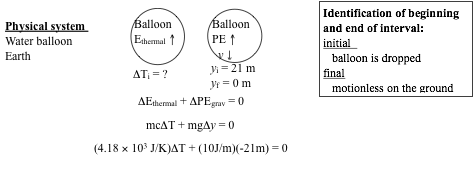
\includegraphics[width=.6\textwidth]{U2/figs/fnt221-5.png}
	\end{center}
}
\begin{FNTenv}
	\label{fnt2.2.1-5}

Christine drops a water balloon from the top of the Science Building. Let's assume that the balloon does not break when it strikes the ground. There are many questions we could ask about this situation. To answer any of them, it makes sense to model the Energy dynamics of the scenario first. Let's do that and then answer some particular questions!

\begin{enumerate}[(a)]
	\item \label{fnt2.2.1-5a} Create a particular model for this phenomenon by making an \EnergyDiagram{} for the process that takes place from the time the water balloon is dropped until it is motionless on the ground. Consider the indicators to determine what energy systems must be present/can be excluded. Have you included enough systems?
	\item If the water balloon falls a distance of \unit[21]{m}, what is the maximum temperature rise of the water balloon due to its being dropped? (Does you answer seem reasonable? Why or why not? It may help to check your units.)
	\item Is there anything that prohibits the water balloon from suddenly cooling off to its original temperature and leaping \unit[21]{m} into the air? From the random nature of thermal energy, why do you think we never see this happen? Respond {\em briefly}.
\end{enumerate}
\end{FNTenv}

\noindent Eventually, Christine grows tired of throwing and dropping things. She goes back into the Science Building to play with a mass that's hanging on a spring in one of the laboratory rooms.

\note{\FNTs~\thechapter-\ref{fnt2.2.1-6}}{
Their main difficulty with this \FNT{} seems to be with the initial and final conditions. For example, it is not necessarily obvious to some of them that ``�moving down through equilibrium�'' means at the equilibrium position.
\\[0.25in]
part a) Energy system diagram- 	
Initial values of indicators: mass at equilibrium position ($x_i$ = 0), with speed zero; 
Final values of indicators: mass 7.1 cm from equilibrium ($x_f$ = 7.1 cm.), with speed zero.  
Physical system is open, with work entering.
$W = \Delta PE_{spring-mass} \to  W = +5 \times 10^{-4}$ J
\\[0.25in]
parts b1 \& b2
Energy system diagram- 	
Initial values of indicators: mass 7.1 cm from equilibrium ($x_i$= 7.1), with speed zero;
Final values of indicators: mass at equilibrium ($x_f$= 0 cm.), with speed unknown.  
Physical system is closed.
\\[0.25in]
parts b3
Energy system diagram- 	
Initial values of indicators: At x = 7.1 cm, with speed zero, or x = 0, with speed = 6 cm/s.
Final values of indicators: xf = 5.0 cm.), with speed unknown.  
Physical system is closed.
}

\begin{FNTenv}
	\label{fnt2.2.1-6}

Christine's mass-spring system consists of a \unit[250]{g} mass hanging from a spring with a spring constant $k = \unitfrac[0.182]{J}{m^2}$. She pulls the mass down \unit[7.1]{cm} from its equilibrium position and then releases it from rest.

\begin{enumerate}[(a)]
	\item How much work did Christine do when she pulled the spring down from its equilibrium position? Assume that the mass was at rest before she pulled it down, and before it was released. (Use the \EnergyInteractionModel{}, {\em not} the expression $W = F_\text{avg} \cdot \Delta x$, to determine the work.)
	\label{fnt2.2.1-6a}
	\item Create a particular model (construct an \EnergyDiagram{}) for each of the following final conditions to predict the speed of the mass after it is released, and when it is:
	\label{fnt2.2.1-6b}
	\begin{enumerate}[(i)]
		\item moving up through the equilibrium position,
		\label{fnt2.2.1-6b1}
		\item moving down through equilibrium, and
		\label{fnt2.2.1-6b2}
		\item \unit[5.0]{cm} below the equilibrium position, moving down.
		\label{fnt2.2.1-6b3}
	\end{enumerate}
\end{enumerate}
\end{FNTenv}


\begin{center}\noindent\textbf{Each group is responsible for putting one of the following on the board.\\ Write so that all other groups can easily follow your presentation!}\end{center}


\noindent\framebox[1.1\width][c]{\textbf{Group 1}}\\

\noindent \hyperref[fnt2.2.1-1]{\FNTs~\thechapter-\ref{fnt2.2.1-1}} \& \hyperref[fnt2.2.1-4]{\FNTs~\thechapter-\ref{fnt2.2.1-4}} (\unit[\textless 5]{min}) 
 
 \begin{itemize}
 	\item[\textbf{Read:}] You should already have used the principle of energy conservation to develop an equation for the change in height of a ball thrown straight up in the air (from \hyperref[act2.2.1b]{Activity~\ref{act2.2.1b}}).
	
	\item[\textbf{Do:}] Write a sentence or two explaining what fundamental feature of the \EnergyInteractionModel{} ``accounts for'' why changing the location of $y = 0$ does not change your calculation of the ball's maximum height above the floor. [\textbf{Hint:} think about the general form of the algebraic expression of energy conservation.]
\end{itemize}

\noindent
\hyperref[fnt2.2.1-2]{\FNTs~\thechapter-\ref{fnt2.2.1-2}}   (\unit[\textless 5]{min})

\begin{itemize}
	\item[\textbf{Read:}] When you model the process described in \ref{fnt2.2.1-2} in two different ways, i.e., using an interval corresponding to the overall process in versus splitting the overall process into two contiguous pieces with separate intervals corresponding to each part, you should get the same result for the speed of the ball at \unit[4]{m} above the floor.
	
	Check with your instructor for the correct numerical answer.
	
	\item[\textbf{Do:}] In terms of the \EnergyInteractionModel{}, why is it not necessary to divide the overall process into two pieces in order to find the speed of the ball at \unit[4]{m} above the floor falling down? 		 
\end{itemize}


\noindent\framebox[1.1\width][c]{\textbf{Group 2}}\\

\noindent
\hyperref[fnt2.2.1-3]{\FNTs~\thechapter-\ref{fnt2.2.1-3}}  (\unit[\textless 10]{min})\\

\noindent Construct one or two \EnergyDiagrams{} that you can use to explain how you know that an object thrown vertically upward will have the same speed as it comes down through any point that it had going up through that same point.\\


\noindent\framebox[1.1\width][c]{\textbf{Group 3}}\\

\noindent
\hyperref[fnt2.2.1-5]{\FNTs~\thechapter-\ref{fnt2.2.1-5}} (\unit[\textless 10]{min})\\

\noindent Construct a complete \EnergyDiagram{} for the process described in \hyperref[fnt2.2.1-5a]{Part~(\ref*{fnt2.2.1-5a})} of this \FNT{}.\\


\noindent\framebox[1.1\width][c]{\textbf{Group 4}}\\

\noindent
\hyperref[fnt2.2.1-6a]{\FNTs~\thechapter-\ref*{fnt2.2.1-6}, Part~(\ref*{fnt2.2.1-6a})} 	(\unit[\textless 10]{min})\\

\noindent Construct a complete \EnergyDiagram{} for the process described in \hyperref[fnt2.2.1-6a]{Part~(\ref*{fnt2.2.1-6a})} of this \FNT{}.\\


\noindent\framebox[1.1\width][c]{\textbf{Group 5}}\\

\noindent\hyperref[fnt2.2.1-6b1]{Parts~b(i) \& b-(ii)} (\unit[\textless 10]{min})\\

\noindent Construct a complete \EnergyDiagram{} for the process described in \hyperref[fnt2.2.1-6b1]{\FNTs~\thechapter-Parts~(b)-(i)} and \hyperref[fnt2.2.1-6b2]{(b)-(ii)} of this \FNT{}.\\


\noindent\framebox[1.1\width][c]{\textbf{Group 6}}\\

\noindent\hyperref[fnt2.2.1-6b3]{\FNTs~\thechapter-\ref*{fnt2.2.1-6}, Part~b(iii)} (\unit[\textless 10]{min})\\

\noindent Construct a complete \EnergyDiagram{} for the process described in \hyperref[fnt2.2.1-6b3]{Part~b(iii)} of this \FNT{}.\\

\WCD